%% SOURCE: experiments/010-kuzmin-tmi/scripts/inference_4_gene_selection.py (roster, results/inference_4/sizing.json), inference_4_generate_triples.py (space, results/inference_4/generation_summary.json), equivariant_cell_graph_transformer_inference_4.py (SLURM jobs 1585-1596), inference_4_rank.py (ranking, results/inference_4/rank_summary.json and top_triples.csv)

\section{inference\_4: metabolism crossed with regulation\secstatus{todo}}

\texttt{inference\_1} covered 324 of the 1{,}161 yeast-GEM genes with no constraint
on how a triple mixed its sources, and its positive tail rested on genes measured
under a single screen. The replacement names its axes and gates its support.

\subsection{The space\secstatus{todo}}

A triple carries 1 to 2 metabolic genes and 1 to 2 regulators, so every prediction
is about regulation acting on metabolism. yeast-GEM 9.0.2 supplies 1{,}161
metabolic genes; TFLink supplies 317 regulators and the SGD regulatory graph 476,
overlapping in 25. After the \texttt{inference\_1} filters, drop SGD-essential,
drop single-mutant fitness below 0.9, drop mitochondrial, 934 genes remain: 676
metabolic, 273 regulator, 15 both.

Support is a screen count, not presence, and the difference is the whole point.
841 of the 934 appear somewhere in the Kuzmin trigenic data, so requiring presence
removes 0.08 percent of the space. 191 clear 50 distinct query screens. Requiring
at least one such gene gives \textbf{41{,}877{,}232} triples, which two independent
derivations agree on: a closed form over gene classes, and the generator's own
enumeration.

Twelve SLURM jobs, three checkpoints at four contiguous shards each, ran in about
2 hours 40 minutes per shard across four GPUs. Every shard file is complete,
strictly ordered and correctly offset, so the four concatenate into dataset order.

\subsection{The checkpoints disagree, so no single tail is reportable\secstatus{todo}}

\begin{table}[H]
\centering
\footnotesize
\begin{tabular}{lrrrrr}
\toprule
Predicted $\tau >$ & M01 & M02 & M03 & Ensemble mean & All three \\
\midrule
$+0.08$ & 449{,}239 & 192{,}355 & 86{,}280 & 43{,}663 & 2{,}906 \\
$+0.12$ &  92{,}127 &  50{,}443 & 19{,}656 & 10{,}518 &   831 \\
$+0.16$ &  33{,}969 &  18{,}794 &  7{,}710 &  4{,}495 &   432 \\
$+0.20$ &  15{,}844 &   8{,}746 &  4{,}231 &  2{,}284 &   272 \\
$+0.30$ &   4{,}611 &   2{,}441 &  1{,}633 &    739 &   152 \\
\bottomrule
\end{tabular}
\caption{Tail size by checkpoint over 41{,}877{,}232 triples. Validation Pearson
is 0.4520, 0.4472 and 0.4619 respectively, so the models are of comparable
quality and still differ fivefold at $+0.08$. Generated by
\protect\file{experiments/010-kuzmin-tmi/scripts/inference\_4\_rank.py}.}
\end{table}

M01 calls five times as many positives as M03 at the $+0.08$ cut, and requiring
all three to clear it removes 99.3 percent of M01's list. The ranking statistic is
therefore the ensemble mean, with the across-checkpoint standard deviation carried
beside every entry.

\subsection{What survives consensus\secstatus{todo}}

A fraction of 41.9 million is not a number anyone can hold, so the counts matter
more than the rates. Requiring every checkpoint to clear the cut, rather than
their mean, is the only basis a panel should be drawn from.

\begin{table}[H]
\centering
\footnotesize
\begin{tabular}{lrrr}
\toprule
Cut & Ensemble mean & All three above & Share of the space \\
\midrule
$>+0.08$ & 43{,}663 & 2{,}906 & 0.0069\% \\
$>+0.12$ & 10{,}518 &   831 & 0.0020\% \\
$>+0.16$ &  4{,}495 &   432 & 0.0010\% \\
$>+0.20$ &  2{,}284 &   272 & 0.0006\% \\
$>+0.30$ &    739 &   152 & 0.0004\% \\
\bottomrule
\end{tabular}
\caption{Consensus counts over 41{,}877{,}232 triples. \textbf{432} clear the
strong tier at $+0.16$ on all three checkpoints, and 152 clear $+0.30$. Generated
by \protect\file{experiments/010-kuzmin-tmi/scripts/inference\_4\_rank.py}.}
\end{table}

\subsection{The support gate did what it was built to do\secstatus{todo}}

This is the one place the new design beats the old outright. Fully supported
triples, all three genes measured under at least 50 screens, are 1.8 percent of
the space and \textbf{10.8 percent} of the top 500, a sixfold enrichment.
Two-supported triples are 20.9 percent of the space and 51.8 percent of the head.
The ranking prefers evidence rather than avoiding it, which is the reverse of
\texttt{inference\_1}, where the tail concentrated on single-screen genes and
collapsed 9.6-fold once they were removed.

476 of the top 500 are positive under all three checkpoints.

\subsection{The head is regulatory, not metabolic\secstatus{todo}}

Triple composition says nothing: 2-metabolic triples are 71.2 percent of the
space and 70.4 percent of the top 500, which is the same to within a percentage
point. The compositional constraint is satisfied identically inside and outside
the head.

The genes carrying the head do differ. 79 genes appear in the top 500: 46
metabolic, 32 regulator, 1 both. Against a roster that is 661 metabolic, 258
regulator and 15 both, regulators are $1.47\times$ enriched among the genes the
model puts at the top, 40.5 percent of head genes against 27.6 percent of the
roster.

So the ranking is not selecting metabolic triples over regulatory ones, it is
selecting particular regulators to pair with metabolism. Which regulators is
answered in panel f and is the concern below.

\subsection{Two reasons not to build from this list yet\secstatus{todo}}

\pfstep{The head is a clique.} 79 distinct genes carry the top 500, out of a
934-gene roster, and 76.4 percent of those triples contain one of just six genes.
\texttt{YPL181W} alone appears in 24 percent. A ranked list that is really a claim
about six genes is not a claim about 41.9 million triples, and this is the shape
that produced the previous panel.

\pfstep{The magnitudes are extrapolation.} The top ensemble mean is $+2.33$. The
measured training labels span $[-1.08, +1.13]$ with a standard deviation of 0.063,
so the leader sits at 37 label standard deviations and roughly twice the largest
value ever observed. The predicted standard deviation across the space is 0.021,
a third of the label spread, which is the ordinary regression-to-the-mean
signature and means these numbers are ranks rather than calibrated $\tau$.

Neither observation says the ordering is wrong. Both say the magnitudes carry no
weight, and that a panel drawn from the head would be a test of six genes.

Every number here is also conditional on a split the model has not been refit on.
The additive null falls from 0.400 to $0.127 \pm 0.033$ under a query-pair-disjoint
split, and the transformer has never been retrained there.

\begin{figure}[H]
\centering
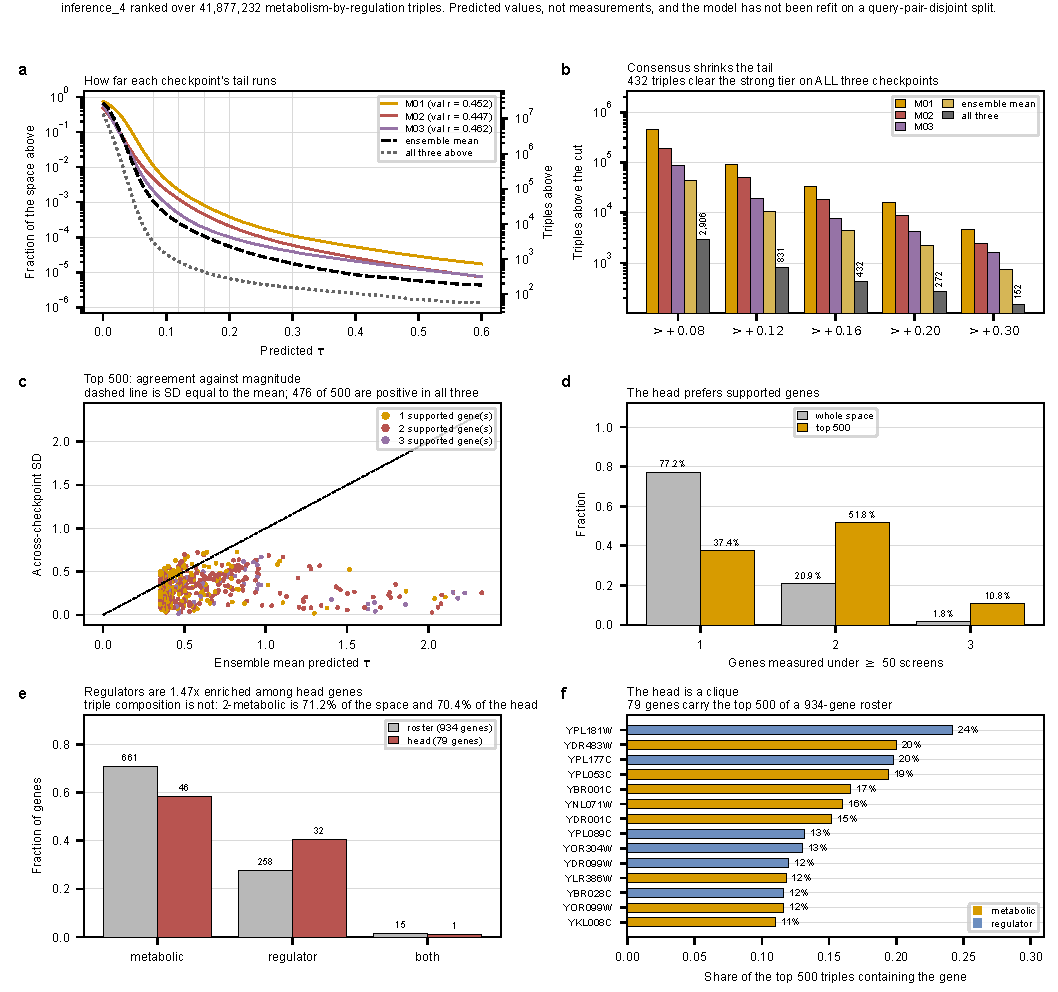
\includegraphics[width=\linewidth]{figures/inference_4_rank.pdf}
\caption{\textbf{a}, how far each checkpoint's tail runs, with absolute counts on
the right axis. \textbf{b}, triples above each cut per checkpoint, for the
ensemble mean, and for consensus across all three. \textbf{c}, agreement against
magnitude for the ranked head, colored by how many of a triple's genes are
screen-supported. \textbf{d}, support composition of the head against the whole
space. \textbf{e}, role of the genes carrying the head against the roster.
\textbf{f}, share of the top 500 containing each of the 14 most frequent genes,
colored by role. Generated by
\protect\file{experiments/010-kuzmin-tmi/scripts/inference\_4\_rank.py}.}
\end{figure}
